% Created 2021-01-29 Fri 15:35
% Intended LaTeX compiler: pdflatex
\documentclass[11pt]{article}
\usepackage[utf8]{inputenc}
\usepackage[T1]{fontenc}
\usepackage{graphicx}
\usepackage{grffile}
\usepackage{longtable}
\usepackage{wrapfig}
\usepackage{rotating}
\usepackage[normalem]{ulem}
\usepackage{amsmath}
\usepackage{textcomp}
\usepackage{amssymb}
\usepackage{capt-of}
\usepackage{hyperref}
\documentclass{article}
\usepackage{here}
\usepackage{xcolor}
\usepackage[margin=3.0cm]{geometry}
\usepackage{amsmath}
\usepackage{parskip}
\renewcommand\arraystretch{1.4}
\documentclass[12pt]{report}
\author{Fatih Kaan Salgır - 171044009}
\date{}
\title{CSE 241 Homework 7}
\hypersetup{
 pdfauthor={Fatih Kaan Salgır - 171044009},
 pdftitle={CSE 241 Homework 7},
 pdfkeywords={},
 pdfsubject={},
 pdfcreator={Emacs 27.1 (Org mode 9.3.7)}, 
 pdflang={English}}
\begin{document}

\maketitle

\section{GUI Design}
\label{sec:org24faa90}
\begin{itemize}
\item \texttt{boardPanel} is Jpanel with \texttt{GridLayout}
\item For identation empty \texttt{JLabel}'s are used
\item Each cell is a \texttt{JButton} with some cutomization

\item To run:
\end{itemize}
\begin{verbatim}
javac *.java
java Main
\end{verbatim}

\begin{figure}[H]
\centering
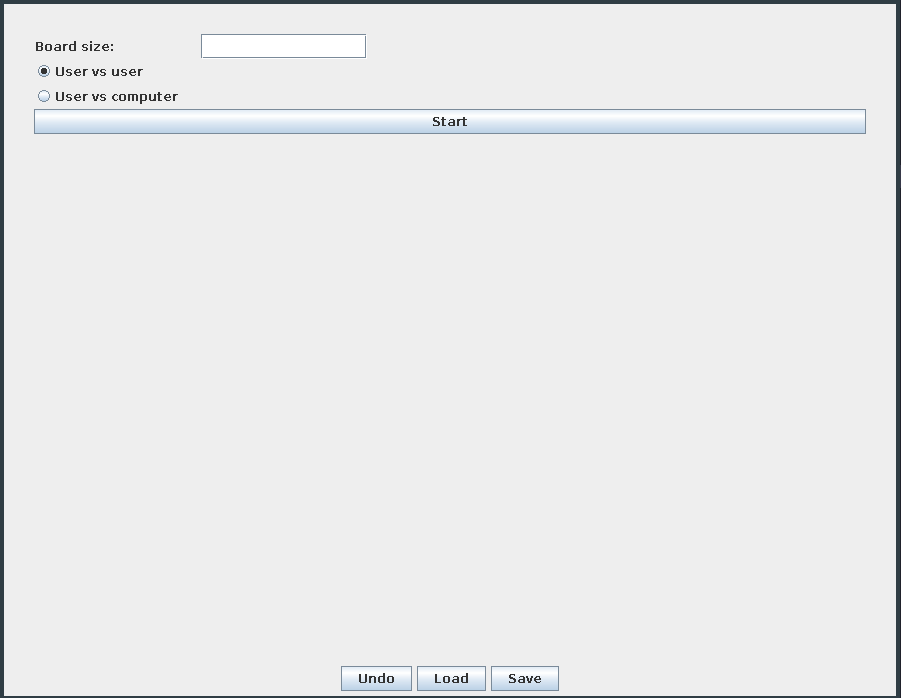
\includegraphics[width=300px]{GUI_Design/2021-01-29_14-49-20_screenshot.png}
\caption{First run of the program}
\end{figure}


\begin{figure}[H]
\centering
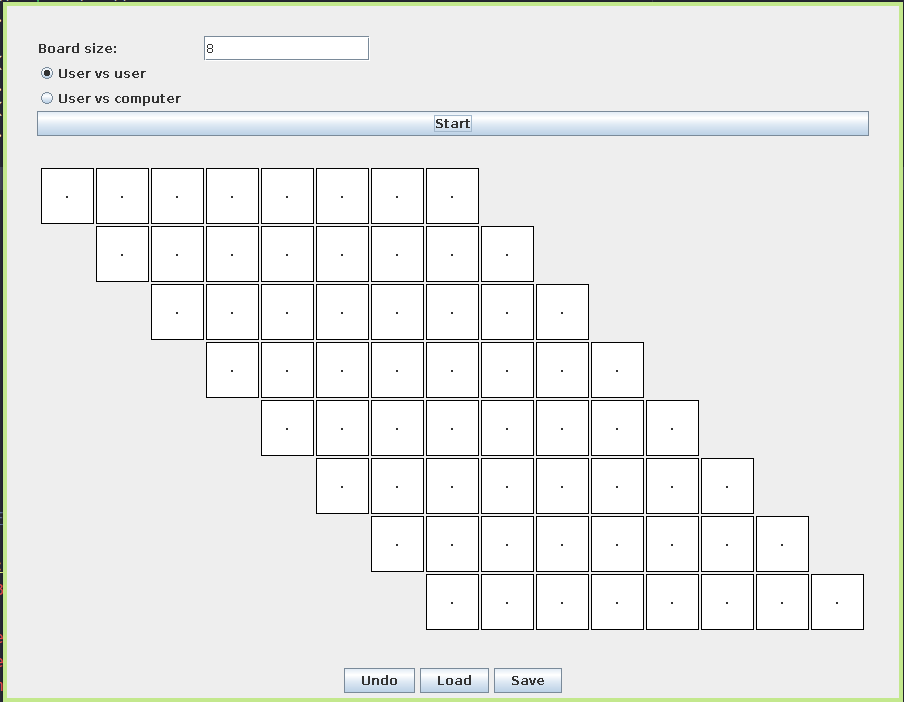
\includegraphics[width=300px]{GUI_Design/2021-01-29_14-57-47_screenshot.png}
\caption{Example 8x8 empty board}
\end{figure}

\begin{figure}[htbp]
\centering
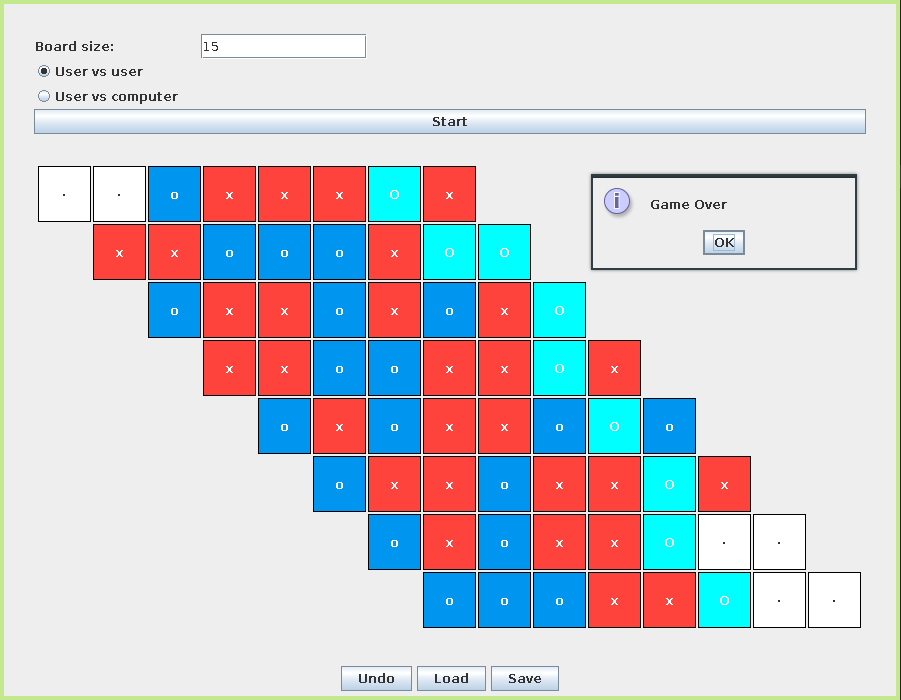
\includegraphics[width=300px]{GUI_Design/2021-01-29_14-59-26_screenshot.png}
\caption{Win situation with blue user. Path highlighted}
\end{figure}


\begin{figure}[H]
\centering
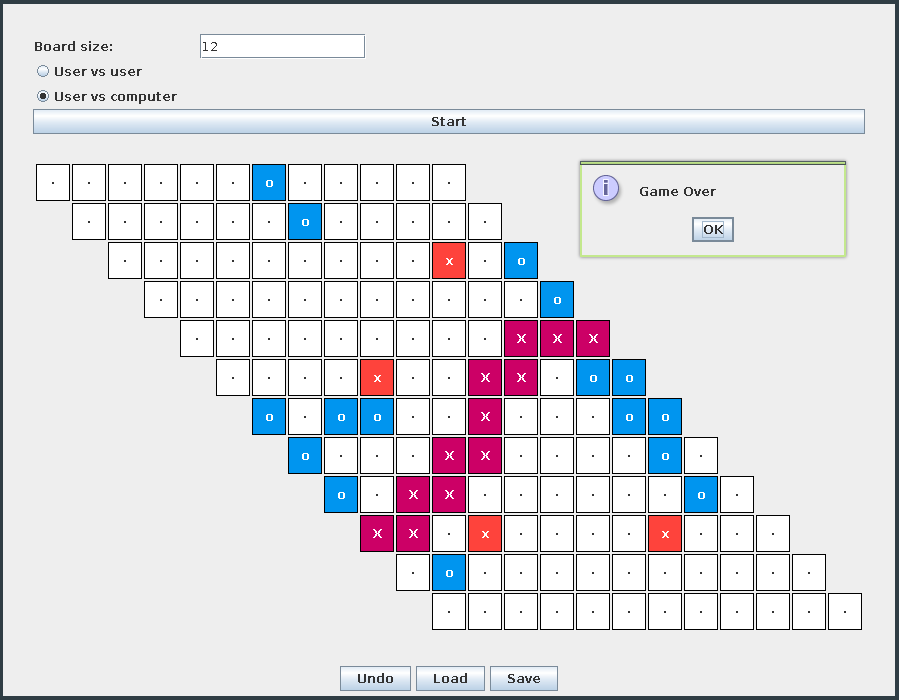
\includegraphics[width=.9\linewidth]{GUI_Design/2021-01-29_15-05-55_screenshot.png}
\caption{Win situation with red user on 12x12 board.}
\end{figure}


\section{File format}
\label{sec:org6167ce2}
Example 8x8 board, user vs user saved file:
\begin{verbatim}
boardSize:8
vsComputer:false
board:..........x.o....o..xo...x........o..ox...x.........o.x..xo.....
nextTurn:x
history.size:14
history:1,3 5,2 2,5 4,1 2,1 1,2 4,2 2,4 6,4 4,6 6,6 2,7 1,7 5,4 
\end{verbatim}

\section{User Input Validity}
\label{sec:orga9a33b0}

\subsection{Board size}
\label{sec:orgcc3b2a5}
I have chosen the maximum limit of board size is 20; since it started to look unreadble after that point.

\begin{center}
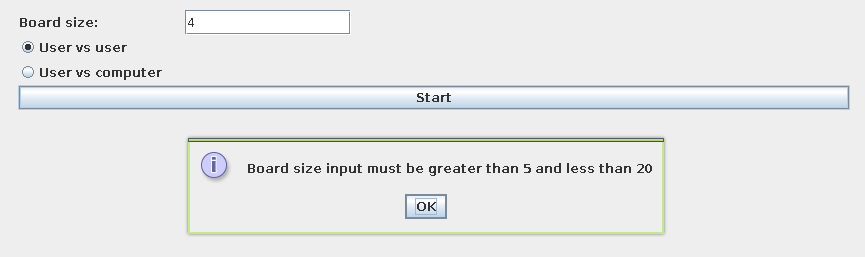
\includegraphics[width=.9\linewidth]{User_Input_Validity/2021-01-29_14-50-22_screenshot.png}
\end{center}

\subsection{Load File}
\label{sec:orgf8ee42d}
Empty input or file is not found in the directory:

\begin{center}
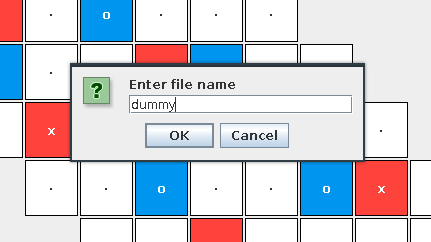
\includegraphics[width=300px]{User_Input_Validity/2021-01-29_14-55-39_screenshot.png}
\end{center}
\begin{center}
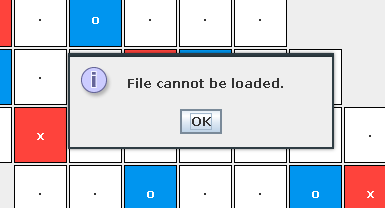
\includegraphics[width=300px]{User_Input_Validity/2021-01-29_14-56-01_screenshot.png}
\end{center}

\begin{itemize}
\item After win, buttons become unclickable.
\end{itemize}

\section{Notes}
\label{sec:org15936b9}

\begin{itemize}
\item Undo after load works.
\item Undo after a win works.
\end{itemize}
\end{document}